\chapter{Noncollapsing}

Noncollapsing in mean curvature flow is a powerful result which gives a geometric idea about the structure of singularities. It can be used to rule out certain singularity profiles for mean convex mean curvature flow. 

\section{Inscribed curvature}

Let $ \mathcal{M} \subset \Rn $ be a smooth hypersurface which is the boundary of an open set $ \Omega \subset \Rn $. For $ x \in \mathcal{M} $, we want to find the radius of the largest inscribed sphere in $ \mathcal{M} $ touching it at $ x $. For any $ y \in \mathcal{M}\backslash \{x\} $, the radius of the sphere passing through $ x $ and $ y $ and touching $ \mathcal{M} $ at $ x $ is given by \begin{equation}
    r(x,y) = \frac{||x-y||^{2}}{2\left< x-y,\nu(x) \right>}
\end{equation}
where $ \nu(x) $ is the outward unit normal vector of $ \mathcal{M} $ at $ x $. The inverse of the radius is the \textbf{extrinsic ball curvature} $ k : \mathcal{M} \times \mathcal{M} \backslash \{(x,x) : x \in \mathcal{M}\} \to \R $ defined by \begin{equation}
    k(x,y) = \frac{2 \left< x-y,\nu(x) \right>}{||x-y||^{2}}.
\end{equation} 
Now for each point $ x \in \mathcal{M} $, we can get the radius of the largest inscribed sphere touching $ \mathcal{M} $ at $ x $  which we call the \textbf{inradius} function $r :  \mathcal{M}  \to (0,\infty]$ given by %and i To get the \textbf{inradius} $ r : \mathcal{M} \to (0, \infty] $ which would be radius of the largest sphere touching $ \mathcal{M} $ at the given point and inscribed in $ \mathcal{M} $, we take the infimum over all points $ y \in \mathcal{M}\backslash \{x\} $ to get 
\begin{equation}
    r(x) = \inf_{{y \in \mathcal{M}\backslash \{x\}}} r(x,y).
\end{equation}
Similarly, the \textbf{inscribed curvature} $ k : \mathcal{M} \to [0, \infty) $  is obtained by the reciprocal of the inradius, so \begin{equation}
    k(x) = \frac{1}{r(x)} = \sup_{y \in \mathcal{M}\backslash \{x\}} k(x,y).%\sup_{y \in \mathcal{M}\backslash \{x\}} \frac{2\left< x-y,\nu(x) \right>}{||x-y||^{2}}
\end{equation}
The inscribed curvature is greater than the largest principal curvature, which can be proved in the following fashion. 
\begin{lemma}
    Let $ \mathcal{M} $ be an embedded hypersurface in $ \Rn $ and the inscribed curvature be defined as above. Then for any point $ x \in \mathcal{M} $,
    \[ k(x) \ge \kappa_{n}(x) \]
    where $ \kappa_{1}(x) \le \ldots \le \kappa_{n}(x) $ are the principal curvatures of the hypersurface at the point $ x  $.
\end{lemma}
\begin{proof}
    TO DO
\end{proof}
\begin{figure}[h]
    \centering
    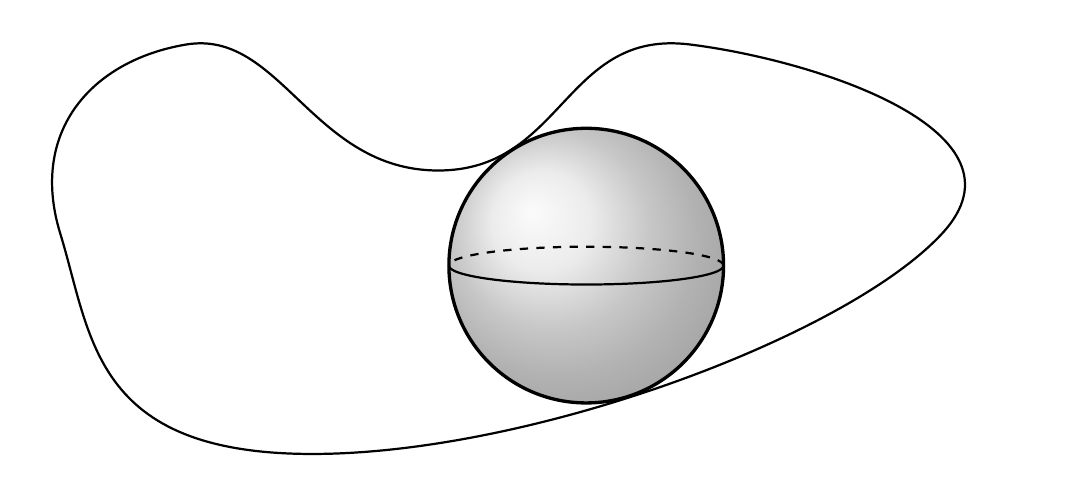
\begin{tikzpicture}[scale=0.8]
        \draw [smooth cycle, tension=0.9, thick] plot coordinates{(2,1) (6,3) (10,0) (0,-3.5) (-4,0) (-2,3)};
        \shade [ball color = gray!40, opacity = 0.5] (4.35,-0.51) circle (2.18cm);
        \draw [very thick](4.35,-0.51) circle (2.18cm);
        \draw [thick](2.17, -0.51) arc (180:360:2.18 and 0.3);
        \draw[thick, dashed] (6.53,-0.51) arc (0:180:2.18 and 0.3);
    \end{tikzpicture}
    \caption{Inscribed sphere of maximum radius}
\end{figure}

\begin{defn}
    Let $ \mathcal{M} $ be a mean convex hypersurface bounding an open set $ \Omega \subset \Rn$, so $ \partial \Omega = \mathcal{M} $. We say that $ \mathcal{M} $ is \textbf{$ \alpha $-noncollapsed}  if for every $ x \in \mathcal{M} $ there exists an open ball $ B $ of radius $ \frac{\alpha}{H(x)} $ touching $ \mathcal{M} $ at $ x $ and contained entirely in $ \Omega $. In terms of inscribed curvature, this is same as the inequality \begin{equation}
        k(x) \le \frac{1}{\alpha} H(x) \quad \text{ for all} \quad x \in \mathcal{M}.
    \end{equation}
\end{defn}
We will prove in the following section that noncollapsing is preserved under mean curvature flow.
%\begin{thm}[Noncollapsing]
    %Let $ X: M^{n} \times [0,T) \to \Rn $ be a smooth solution of the mean curvature with $ X(\cdot, 0) = \mathcal{M}_{0} $ compact and $ \alpha $-noncollapsed. Then $ X(\cdot,t) = \mathcal{M}_{t} $ is $ \alpha $-noncollapsed for all $t \in [0,T)  $.  
%\end{thm}
\section{Differential inequality for inscribed curvature}

Following \cite{andrews2022extrinsic,brendle2015sharp} the time evolution equation of inscribed curvature satisfies an inequality which implies noncollapsing. The main difficulty of the proof lies in manipulating the complicated time derivative of $ k $ to get the useful gradient terms with signs. 

\begin{thm}\label{gradnoncollapsing}
    Let $ X : M^{n} \times [0,T) \to \Rn $ be a smooth solution of the mean curvature flow with $ \mathcal{M}_{0} $ properly embedded. Then \begin{equation}
        \frac{\partial k}{ \partial t} \le \Delta k + |A|^{2}k -2 \sum_{\kappa_{i}<k} \frac{(\nabla_{i}k)^{2}}{k- \kappa_{i}} \label{gradientnoncollapsing}
    \end{equation}
    where the inequality holds in the viscosity sense. 
\end{thm}
\begin{comment}
    Before that we will show that  
\begin{lemma}
    The inscribed curvature satisfies 
    \[ k(x) \ge \lim_{y \to x} \sup k(x,y) = \kappa_{n}(x) \]
    where $ \kappa_{1} \le \ldots \le \kappa_{n} $ denotes the principal curvatures of $ \mathcal{M} $. 
\end{lemma}
\end{comment}
\begin{proof}[\cref{gradnoncollapsing}]
    For any given point $ (x_{0},t_{0}) \in \mathcal{M} \times [0,T) $, either of the two cases occur
    \begin{enumerate}
        \item $ k(x_{0},t_{0}) = \lim_{y \to x_{0}} k(x_{0},y,t_{0}) $, or 
        \item $ k(x_{0},t_{0}) = k(x_{0}, y_{0},t_{0}) $ for some $ y_{0} \in \mathcal{M}_{t_{0}} \backslash \{x_{0}\} $.
    \end{enumerate}

    We will be concentrating only on the second case which happens on an open subset of spacetime, where the supremum is achieved from a sphere touching the hypersurface at two separate points. The first case occurs on a set with measure zero and is covered in Proposition 12.8 in \cite{andrews2022extrinsic}.
    
    Let $ U $ be an open neighborhood of $ x_{0} $ and $ \psi : U \times (t_{0}-\alpha,t_{0}] \to \R $ be a smooth function such that $ \psi(x_{0},t_{0}) = k(x_{0},t_{0}) $ and $ \psi(x,t) \ge k(x,t) $ for all $ (x,t) \in U \times (t_{0}-\alpha,t_{0}] $. We want to prove\begin{equation}
        \frac{\partial \psi}{\partial t} \le \Delta \psi + |A|^{2}\psi - 2 \sum_{i=1}^{n} \frac{ (\nabla_{i}\psi)^{2}}{\psi-\kappa_{i}}. \label{psi}
    \end{equation}
    Define \begin{align}
        Z(x,y,t) & = \frac{1}{2}\psi(x,t)|X(x,t)-X(y,t)|^{2} - \left< X(x,t) - X(y,t), \nu(x,t) \right>
    \end{align}
    which can be further simplified to \begin{equation*}
        Z(x,y,t) = \frac{|X(x,t)-X(x,t)|^{2}}{2}(\psi(x,t) - k(x,t)) %  \quad \text{ if }  x \neq y
    \end{equation*}
    for all $ x \neq y $. Observe that $ Z(x_{0},y_{0},t_{0}) = 0 $  and $ Z(x,y,t) \ge 0 $ for all $ (x,y,t) \in U \times M \times (t_{0}-\alpha,t_{0}] $ from the hypothesis on $ \psi $. 

    The space derivatives in local coordinates are 
    \begin{align}
        \frac{\partial Z}{ \partial x_{i}}  & =  \frac{1}{2} \frac{\partial \psi}{\partial x_{i}}(x,t)|X(x,t) - X(y,t)|^{2} + \psi(x,t)\left< X(x,t)-X(y,t), \frac{\partial X}{\partial x_{i}}(x,t) \right> \nonumber \\
        & \quad - h_{i}^{k}(x,t)\left< X(x,t)-X(y,t), \frac{\partial X}{\partial x_{k}}(x,t) \right> \label{Zxi}
    \end{align}
    and \begin{align}
        \frac{\partial Z}{\partial y_{i}} = - \psi(x,t)\left< \frac{\partial X}{\partial y_{i}}(y,t), X(x,t) - X(y,t) \right> + \left< \frac{\partial X}{\partial y_{i}}(y,t) , \nu(x,t)\right> \label{Zyi}
    \end{align}
    Choose normal coordinates around $ x_{0} $ such that $ h_{ij}(x_{0},t_{0}) $ is diagonal. Then \cref{Zxi} at the minima $ (x_{0},y_{0}) $ gives
    
        %\begin{equation}
        %\left< X(x_{0},t_{0})-X(y_{0},t_{0}), \frac{\partial X}{\partial x_{i}}(x_{0},t_{0}) \right> = -\frac{1}{2} \frac{1}{\psi(x_{0},t_{0})-\kappa_{i}(x_{0},t_{0})} \frac{\partial \psi}{\partial x_{i}}(x_{0},t_{0}) |X(x_{0},t_{0})-X(y_{0},t_{0})|^{2}. \label{psiequation}
    %\end{equation}

    \begin{equation}
        \left< \eta, \frac{\partial X}{\partial x_{i}}(x_{0},t_{0}) \right> = -\frac{1}{2} \frac{1}{\psi(x_{0},t_{0})-\kappa_{i}(x_{0},t_{0})} \frac{\partial \psi}{\partial x_{i}}(x_{0},t_{0}) |X(x_{0},t_{0})-X(y_{0},t_{0})| \label{psiequation}
    \end{equation}
    where $ \eta = \frac{X(x_{0},t_{0})-X(y_{0},t_{0})}{|X(x_{0},t_{0})-X(y_{0},t_{0})|} $. The tangent space at $ y_{0} $ can be obtained by reflection across the hyperplane with normal $ \eta $. In particular, \begin{align}
        \nu(y_{0},t_{0}) &= \nu(x_{0},t_{0}) - 2 \eta \left< \nu(x_{0},t_{0}), \eta \right> \nonumber\\ 
        & = \nu(x_{0},t_{0}) - \psi(x_{0},t_{0})(X(x_{0},t_{0})-X(y_{0},t_{0})). \label{etay}
    \end{align}
    Now we choose normal coordinates around $ y_{0} $, such that the reflection of $ \frac{\partial X}{\partial x_{i}} $ across $ \eta $ is $ \frac{\partial X}{\partial y_{i}} $, so \begin{align}
        \frac{\partial X}{\partial y_{i}} & = \frac{\partial X}{\partial x_{i}} - 2 \eta \left< \frac{\partial X}{\partial x_{i}}, \eta \right>
    \end{align}

    Also,\begin{align}
        \left< \frac{\partial X}{\partial y_{i}}(y_{0},t_{0}), \frac{\partial X}{\partial x_{i}}(x_{0},t_{0}) \right> & = 1-2 \eta \left< \frac{\partial X}{\partial x_{i}}(x_{0},t_{0}), \eta \right>^{2} \label{innerproduct}
    \end{align}


   % Our aim is to get an elliptic partial differential equation for $ Z $ which will prove the inequality for $ \psi $ using maximum principles. 
    Further, calculating the double space derivatives, \begin{align}
        \frac{\partial^{2}Z}{\partial x_{i}^{2}}(x,y,t) & = \frac{1}{2}\frac{\partial^{2} \psi}{\partial x_{i}^{2}}|X(x,t)-X(y,t)|^{2} + 2\frac{\partial \psi}{\partial x_{i}}\left< X(x,t)-X(y,t), \frac{\partial X}{\partial x_{i}} \right> \nonumber \\
        & \quad + \psi \left< \frac{\partial X}{\partial x_{i}}, \frac{\partial X}{\partial x_{i}} \right> + \psi \left< X(x,t)-X(y,t), \frac{\partial^{2} X}{\partial x_{i}^{2}} \right> \nonumber \\
        & \quad - \frac{\partial h_{i}^{k}}{\partial x_{i}}\left< X(x,t)-X(y,t), \frac{\partial X}{\partial x_{k}} \right> - h_{i}^{k}\left< \frac{\partial X}{\partial x_{i}}, \frac{\partial X}{\partial x_{k}} \right>\nonumber \\
        & \quad - h_{i}^{k}\left< X(x,t)-X(y,t), \frac{\partial^{2}X}{\partial x_{i}\partial x_{k}} \right> \label{Zxx}
    \end{align}
    Recall we had chosen normal coordinates at $ x_{0} $ such that the matrix $ h_{ij}(x_{0},t_{0}) $ is diagonal so
    \[ \frac{\partial^{2}X}{\partial x_{i}^{2}} = \Gamma_{ii}^{k}\frac{\partial X}{\partial x_{k}} -h_{ii}\nu = -\kappa_{i}\nu. \]
    Adding the \cref{Zxx} from $ i=1 $ to $ n $, and evaluating it at $ (x_{0},y_{0},t_{0}) $, 

    \begin{align}
        \sum_{i=1}^{n} \frac{\partial^{2}Z}{\partial x_{i}^{2}}(x_{0},y_{0},t_{0}) & = \frac{1}{2} \Delta \psi |X(x_{0},t_{0})- X(y_{0},t_{0})|^{2} - 2 \sum_{i=1}^{n} \frac{\partial \psi}{\partial x_{i}}(x_{0},t_{0})\left< X(x_{0},t_{0})-X(y_{0},t_{0}), \frac{\partial X}{\partial x_{i}} \right> \nonumber\\ 
        & \quad + n \psi + \psi\left<X(x_{0},t_{0})-X(y_{0},t_{0}), -H(x_{0},t_{0})\nu(x_{0},t_{0})  \right> \nonumber\\
        & \quad - \sum_{i=1}^{n} \frac{\partial H}{\partial x_{i}}(x_{0},t_{0})\left< X(x_{0},t_{0})-X(y_{0},t_{0}), \frac{\partial X}{\partial x_{i}} \right>- H(x_{0},t_{0})\nonumber \\
        & \quad + |A(x_{0},t_{0})|^{2}\left< X(x_{0},t_{0})-X(y_{0},t_{0}), \nu(x_{0},t_{0}) \right>
    \end{align}
    where we used the Codazzi equation $ \sum \partial_{i}h_{i}^{k} = \partial_{k}H $ for normal coordinates and the mean curvature vector equation $ \Delta X = -H \nu $. Using  \cref{psiequation} this can be written as, \begin{align}
        \sum_{i=1}^{n} \frac{\partial^{2}Z}{\partial x_{i}^{2}}(x_{0},y_{0},t_{0}) & = \frac{1}{2} \bigg( \Delta \psi(x_{0},t_{0}) + |A(x_{0},t_{0})|^{2}\psi(x_{0},t_{0}) \nonumber \\
        & \quad- \sum_{i=1}^{n} \frac{2}{\psi(x_{0},t_{0})- \kappa_{i}(x_{0},t_{0})}\left( \frac{\partial \psi}{\partial x_{i}}(x_{0},t_{0}) \right)^{2} \bigg)|X(x_{0},t_{0})-X(y_{0},t_{0})|^{2} \nonumber \\
        & \quad - \sum_{i=1}^{n} \frac{\partial H}{\partial x_{i}}(x_{0},t_{0}) \left< X(x_{0},t_{0})-X(y_{0},t_{0}), \frac{\partial X}{\partial x_{i}}(x_{0},t_{0}) \right> \nonumber \\
        & \quad - H(x_{0},t_{0})\psi(x_{0},t_{0})\left< X(x_{0},t_{0})-X(y_{0},t_{0}), \nu(x_{0},t_{0}) \right>\nonumber \\
        & \quad + n \psi(x_{0},t_{0}) - H(x_{0},t_{0}).
    \end{align}
    Now the mixed derivatives are given by
    \begin{align*}
        \frac{\partial^{2} Z}{\partial x_{i}\partial y_{i}}(x,y,t) & = - \frac{\partial \psi}{\partial x_{i}}(x,t)\left< \frac{\partial X}{\partial y_{i}}(y,t), X(x,t)-X(y,t) \right> - \psi(x,t)\left<  \frac{\partial X}{\partial y_{i}}(y,t), \frac{\partial X}{\partial x_{i}}(x,t) \right> \nonumber \\
        & \quad + \left< \frac{\partial X}{\partial y_{i}}(y,t) , \frac{\partial \nu}{\partial x_{i}}(x,t)\right>
    \end{align*}
    Evaluating this at $ (x_{0},y_{0},t_{0}) $ and using \cref{psiequation} and \cref{innerproduct}, we get 
    \begin{align*}
        \frac{\partial^{2} Z}{\partial x_{i}\partial y_{i}}(x_{0},y_{0},t_{0}) & = -  \frac{\partial \psi}{\partial x_{i}}(x_{0},t_{0}) \left< \frac{\partial X}{\partial y_{i}}(y_{0},t_{0}), X(x_{0},t_{0})-X(y_{0},t_{0}) \right>\\
        & - (\psi(x_{0},t_{0})- \kappa_{i}(x_{0},t_{0}))\left< \frac{\partial X}{\partial y_{i}}(y_{0},t_{0}), \frac{\partial X}{\partial x_{i}}(x_{0},t_{0}) \right> \\
        & = \frac{\partial \psi}{\partial x_{i}}(x_{0},t_{0})\left< X(x_{0},t_{0})-X(y_{0},t_{0}), \frac{\partial X}{\partial x_{i}}(x_{0},t_{0}) \right> \\
        & - (\psi(x_{0},t_{0})-\kappa_{i}(x_{0},t_{0}))\left( 1 -2 \eta \left< \frac{\partial X}{\partial x_{i}}(x_{0},t_{0}) \right>^{2} \right) \\
        & = - (\psi(x_{0},t_{0})- \kappa_{i}(x_{0},t_{0}))
    \end{align*}
    For the second order $ y $ derivative, 
    \begin{align*}  
        \frac{\partial^{2} Z}{\partial y_{i}^{2}}(x,y,t) & = - \psi(x,t) \left< \frac{\partial^{2} X}{\partial y_{i}^{2}}(y,t), X(x,t) - X(y,t) \right> - \psi(x,t)\left< \frac{\partial X}{\partial y_{i}}(y,t), - \frac{\partial X}{\partial y_{i}}(y,t) \right> \\
        & \quad + \left< \frac{\partial^{2} X}{\partial y_{i}^{2}}(y,t), \nu(x,t) \right>
    \end{align*}    
    So from \cref{etay} at $ (x_{0},y_{0},t_{0}) $,
    \begin{align}
        \frac{\partial Z}{\partial y_{i}^{2}}(x_{0},y_{0},t_{0}) & =  \psi(x_{0},t_{0})\kappa_{i}(y_{0},t_{0})\left< X(x_{0},t_{0})-X(y_{0},t_{0}), \nu(y_{0},t_{0}) \right>+\psi(x_{0},t_{0}) \nonumber \\
        & \quad - \kappa_{i}(y_{0},t_{0})\left< \nu(y_{0},t_{0}), \nu(x_{0},t_{0}) \right> \nonumber \\
        & =  \psi(x_{0},t_{0})\kappa_{i}(y_{0},t_{0}) \left( \left< X(x_{0},t_{0})-X(y_{0},t_{0}), \nu(x_{0},t_{0}) \right> - \psi(x_{0},t_{0})|X(x_{0},t_{0})-X(y_{0},t_{0})|^{2}\right)\nonumber \\
        & \quad + \psi(x_{0},t_{0}) - \kappa_{i}(y_{0},t_{0})(1- \psi(x_{0},t_{0})\left< X(x_{0},t_{0})-X(y_{0},t_{0}), \nu(x_{0},t_{0}) \right>) \nonumber\\
        & =  \psi(x_{0},t_{0}) - \kappa_{i}(y_{0},t_{0})
    \end{align}

    Now the time derivative is,
    
    \begin{align*}
        \frac{\partial Z}{\partial t}(x_{0},y_{0},t_{0}) & = \frac{1}{2} \frac{\partial \psi}{\partial t}(x_{0},t_{0})|X(x_{0},t_{0})-X(y_{0},t_{0})|^{2} \\
        & \quad + \psi(x_{0},t_{0}) \left< -H(x_{0},t_{0})\nu(x_{0},t_{0})+H(y_{0},t_{0})\nu(y_{0},t_{0}), X(x_{0},t_{0})-X(y_{0},t_{0}) \right>  \\
        &\quad - \left< -H(x_{0},t_{0})\nu(x_{0},t_{0})+H(y_{0},t_{0})\nu(y_{0},t_{0}), \nu (x_{0},t_{0}) \right> \\
        & \quad - \sum_{i=1}^{n} \frac{\partial H}{\partial x_{i}}(x_{0},t_{0}) \left< X(x_{0},t_{0})-X(y_{0},t_{0}), \frac{\partial X}{\partial x_{i}}(x_{0},t_{0}) \right> \\
        & = \frac{1}{2} \frac{\partial \psi}{\partial t}(x_{0},t_{0})|X(x_{0},t_{0})-X(y_{0},t_{0})|^{2} \\
        & \quad - \sum_{i=1}^{n} \frac{\partial H}{\partial x_{i}}(x_{0},t_{0})\left< X(x_{0},t_{0})-X(y_{0},t_{0}), \frac{\partial X}{\partial x_{i}}(x_{0},t_{0}) \right> \\ 
        & \quad -H(x_{0},t_{0})\psi(x_{0},t_{0})\left< X(x_{0},t_{0})-X(y_{0},t_{0}), \nu(x_{0},t_{0}) \right> + H(x_{0},t)-H(y_{0},t_{0})
    \end{align*}
    where $ \nu(x_{0},t_{0}) - \psi(x_{0},t_{0})(X(x_{0},t_{0})-X(y_{0},t_{0})) =\nu(y_{0},t_{0})  $ was used for last equality. Putting together we get the elliptic term, \begin{align*}
        & \frac{\partial Z}{\partial t}(x_{0},y_{0},t_{0}) - \sum_{i=1}^{n}\left( \frac{\partial^{2} X}{\partial x_{i}^{2}} + 2 \frac{\partial^{2}Z}{\partial x_{i}\partial y_{i}} + \frac{\partial^{2} Z}{\partial y_{i}^{2}} \right)(x_{0},y_{0},t_{0}) \\
        & = \frac{1}{2}\bigg( \frac{\partial \psi}{\partial t}(x_{0},t_{0}) - \Delta \psi(x_{0},t_{0}) - |A(x_{0},t_{0})|^{2} \psi(x_{0},t_{0}) \\
        & \qquad \sum_{i=1}^{n} \frac{2}{\psi(x_{0},t_{0})-\kappa_{i}(x_{0},t_{0})}\left( \frac{\partial \psi}{\partial x_{i}}(x_{0},t_{0}) \right)^{2} \bigg)|X(x_{0},t_{0})-X(y_{0},t_{0})|^{2}
    \end{align*}
    As $ (x_{0},y_{0},t_{0}) $ is a local minimum of $ Z $, the left-hand side of previous equation is negative from which the inequality \cref{psi} follows. 
    
    


















\end{proof}
\begin{corollary}
    [Noncollapsing]
    Let $ X: M^{n} \times [0,T) \to \Rn $ be a smooth solution of the mean curvature with $ X(\cdot, 0) = \mathcal{M}_{0} $ compact and $ \alpha $-noncollapsed. Then $ X(\cdot,t) = \mathcal{M}_{t} $ is $ \alpha $-noncollapsed for all $t \in [0,T)  $. 
\end{corollary}
\begin{proof}
    From \cref{gradientnoncollapsing}, it follows that 
    \[ \frac{\partial k}{ \partial t} \le \Delta k + |A|^{2}k.\]
    Recall that the mean curvature $ H $, satisfies \cref{dtH} so the time derivative of the quotient $ \frac{k}{H} $ satisfies \begin{align*}
        \frac{\partial }{\partial t}\left( \frac{k}{H} \right)  & \le \frac{(\Delta k+|A|^{2}k)H - (\Delta H + |A|^{2}H)k}{H^{2}} \\
        & = \Delta \left( \frac{k}{H} \right) + \frac{2}{H}\left< \nabla \left( \frac{k}{H} \right), \nabla H \right>.
    \end{align*}
    Now maximum principle (for viscosity solutions) yields $ \alpha k \le H  $ for all $ t \in [0,T) $. 
\end{proof}